\chapter{Set-Up of Experiment}
%
Some equipment and materials are needed to perform the experiments as seen in \cref{fig:setup}.
%
\begin{figure}[h]
	\centering
	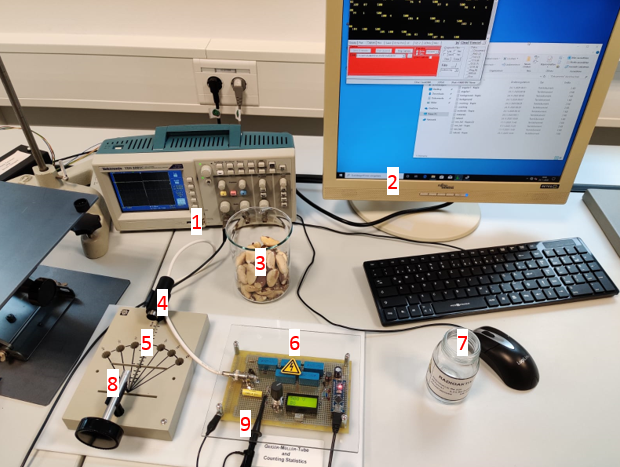
\includegraphics[width=.9\textwidth]{aufbau/setup.PNG} % changed to local path
	\caption[Equipment used.]{Equipment and material required for the experiments.}
	\label{fig:setup} 
\end{figure}
%
\begin{enumerate}
	\item Oscilloscope
	\item Computer running \textsc{RealTerm}
	\item Beaker with Brazil Nuts
	\item \textsc{Geiger-Müller} tube
	\item Mounting plate
	\item Circuit board
	\item Protective container
	\item Radioactive source (\isotope[226]{Ra}, \SI[]{3.3}[]{kBq})
	\item Oscilloscope Probe
\end{enumerate}\par\medskip
%
A detailed view of the circuit board will give \cref{fig:circuit_board}.
%
\begin{figure}[H]
	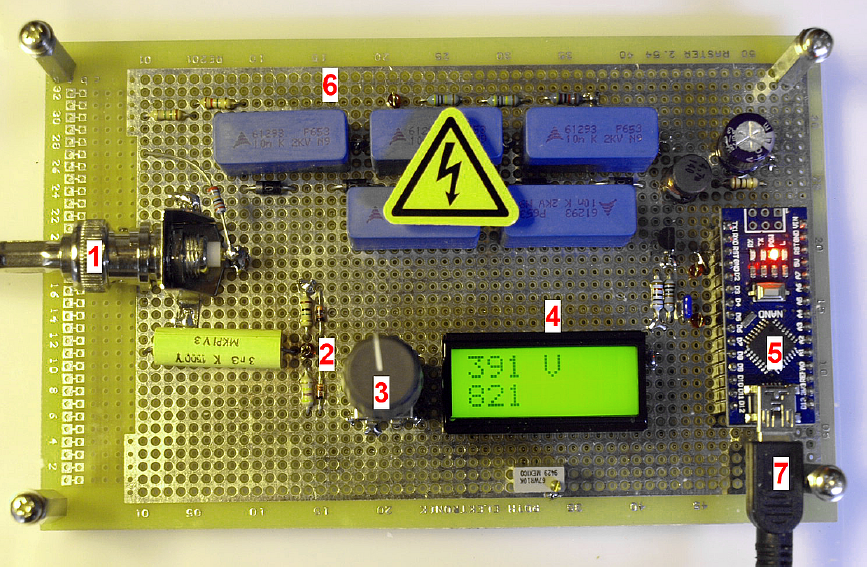
\includegraphics[width=.9\textwidth]{aufbau/circuit_board.png}
	\caption[Close-up of the electronics]{Close-up of the circuit board used \cite[]{AlexanderDorr.GMT}.}
	\label{fig:circuit_board}
\end{figure}
%
\begin{enumerate}
	\item BNC connector
	\item Test point
	\item Potentiometer to adjust the the high-side voltage
	\item LCD
	\item Arduino nano
	\item Boost converter
	\item USB port
\end{enumerate}\par\medskip
%
Using a desktop computer a serial connection via USB is established. A serial monitor - \textsc{RealTerm} - is used to
log the inbound stream send by the MCU. The relevant settings are listed below:
\begin{itemize}
	\item \SI[]{9600}[]{Baud}
	\item On the \texttt{Display} tab, \texttt{Ascii} and \texttt{new Line mode} are checked, \texttt{Direct capture} remains un-checked.
	\item COM-Port as assigned by the OS.
\end{itemize}
%
The data is now continuously sent by the microcontroller. The data is displayed on the screen. A text file is created in
which the data is written and saved. Three columns are displayed. The first column contains the number of the measurement,
the second the counts per \SI[]{10}[]{s} and the third column the present voltage \(U_{GMT}\).\par
To visualize the waveform of the individual signals the probe tip is connected to the test point as seen in \cref{fig:circuit_board}.
The reference lead is connected to one of the nearby stand-offs as they themselfes are connected to ground. On the oscilloscope,
Volts and time per division are adjusted so that a single pulse fills the screen as good as possible.\par
Now the setup is completed and the experiments can be started.